\subsection{Architettura dei simulatori} \label{sec:architettura_simulatori}
Nonostante i simulatori non siano ufficialmente considerati parte integrante del prodotto dalla proponente, il nostro team ha scelto di dedicare alcune risorse alla progettazione di questa componente nell'ambito del progetto didattico. Inoltre, abbiamo deciso di implementare e tenere conto delle possibili logiche dei microcontrollori associati ai sensori IoT, che possono effettuare operazioni per rendere più efficiente l'intero sistema.

Nei paragrafi successivi, verrà presentata l'architettura individuata mediante l'utilizzo di diagrammi delle classi e relative descrizioni rapide. Inoltre, saranno motivate le scelte dei design pattern individuati e le decisioni progettuali rilevanti. Successivamente, per ogni classe, saranno illustrati metodi e attributi.
\subsubsection{Modulo simulatori sensori}
\begin{figure}[H]
    \centering
    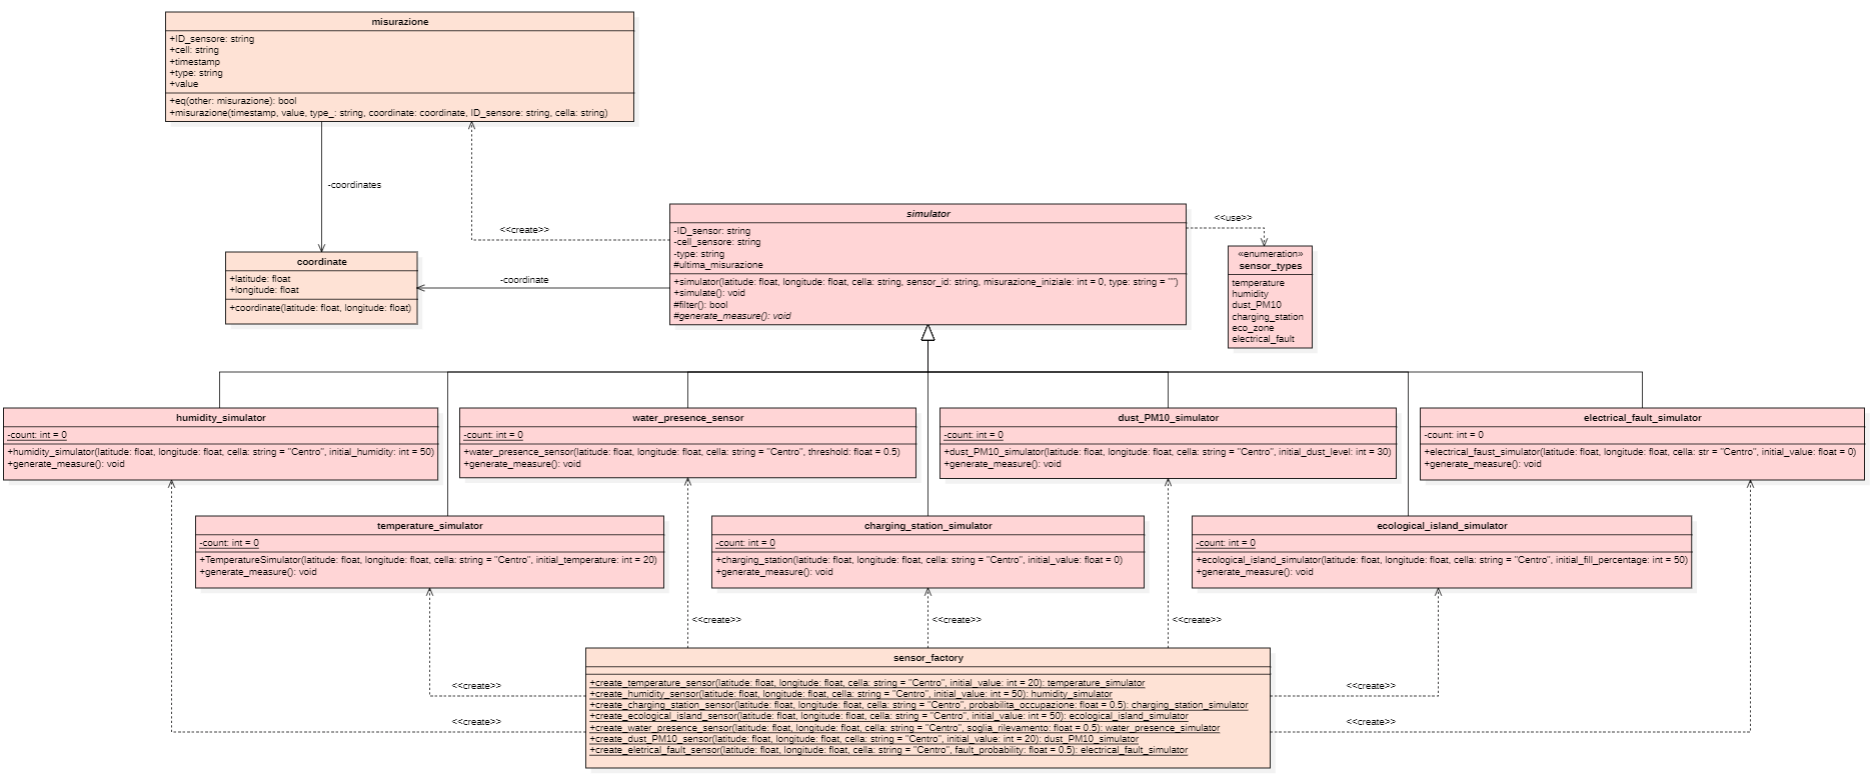
\includegraphics[width=1\textwidth]{../Images/SpecificaTecnica/simulatoriSensori.PNG}
    \caption{Modulo simulatori sensori - innovacity}
    \label{fig: fddf}
\end{figure}
Questo modulo si occupa della generazione di dati di misurazione per diverse tipologie di sensori.

\paragraph{Design pattern Template Method:}

La classe astratta \textit{Simulator} implementa il design pattern \textit{Template Method}. Il metodo \textit{simulate()} fornisce lo scheletro dell'algoritmo per la generazione e la gestione delle misurazioni. Le classi concrete che estendono \textit{Simulator} implementano:
\begin{itemize}
    \item \textbf{Metodo \textit{generate\_measure()}}: per la generazione semi randomica della misurazione associata al tipo di sensore;
    \item \textbf{Metodo \textit{filter()}}: per la logica di filtrazione di misurazioni errate o non attendibili (ad esempio, negative, fuori range o consecutive troppo distanti). Il metodo \textit{filter()} offre un'implementazione di default che lascia passare ogni misurazione senza modifiche.
\end{itemize}

Il design pattern \textit{Template Method} è stato scelto per:
\begin{itemize}
    \item Permettere una facile estensione del sistema con nuovi tipi di sensori che dovranno unicamente implementare la loro logica di generazione delle misurazioni e di filtering se necessario;
    \item Standardizzare i passi per la generazione delle misurazioni, garantendo coerenza e manutenibilità del codice;
    \item Ridurre la duplicazione del codice.
\end{itemize}

Una volta ottenuto lo stato del sensore, esso viene inserito in un oggetto di tipo \textit{Misurazione}. Questo oggetto contiene informazioni di contesto come:
\begin{itemize}
    \item Identificativo del sensore;
    \item Cella della città in cui è presente;
    \item Timestamp della misurazione;
    \item Valore della misurazione;
    \item Coordinate;
    \item Tipologia di misurazione.
\end{itemize}
L'oggetto \textit{Misurazione} viene poi ritornato al chiamante che si occuperà di inviarlo al server \textit{Kafka}.
Un oggetto di tipo \textit{Simulator} verrà assegnato ad ogni \textit{SimulatorThread} che chiamerà ad intervalli regolari il metodo \textit{simulate()} ottenendo appunto la misurazione che invierà al server \textit{Kafka} tramite un modulo apposito e indipendendente.

\paragraph{Design pattern Factory:}
SensorFactory implementa il design pattern \textit{Factory} per la creazione di simulatori dei sensori.
Il pattern FACTORY è un pattern di tipo “Creazionale” secondo la classificazione della GoF.
I pattern di tipo creazionali si occupano della costruzione delle simulazioni dei sensori e delle problematiche che si possono originare, astraggono il processo di creazione degli oggetti, nascondono i dettagli della creazione e rendono i sistemi indipendenti da come gli oggetti sono creati e composti.
Il pattern Factory incapsula la creazione concreta dei sensori, consentendo al client
(l’utilizzatore) di non conoscere i dettagli.


\paragraph{Classi: metodi e attributi}
\begin{itemize}
    \item {\textbf{Classe astratta: \textit{Simulator}}}
        \begin{itemize}
            \item \textbf{Attributi}: 
            \begin{itemize}
                \item \textbf{ID\_sensor:str [private]} - Identificatore univoco del sensore.
                \item \textbf{cella\_sensore:str [private]} - Identificatore della cella del sensore.
                \item \textbf{coordinate:Coordinate [private]} - Coordinate geografiche del sensore.
                \item \textbf{misurazione: T [protected]} - Misurazione corrente del sensore.
                \item \textbf{type:str [private]} - Tipo di sensore.
            \end{itemize}
            \item \textbf{Metodi}:
            \begin{itemize}
                \item \textbf{simulate():Misurazione [public]} - Metodo principale per simulare la generazione di una misurazione.
                Si basa sul design pattern Template Method:
                \begin{enumerate}
                    \item     Chiama generate\_measure() per generare un valore di misurazione.
                    \item     Verifica con filter() se la misurazione è valida (ripete la generazione finché non lo è).
                    \item     Restituisce un oggetto Misurazione con data e ora corrente, valore misurato, tipo di sensore, coordinate e identificativo del sensore.
                \end{enumerate}
                \item \textbf{generate\_measure():None [protected]} - Metodo astratto da implementare nelle classi concrete per generare un valore di misurazione semi-casuale coerente con la tipolgia di sensore da salvare nell'attributo \textit{misurazione}.
                \item \textbf{filter():bool [protected]} - Metodo di filtro per la validazione della misurazione (implementazione di default che accetta sempre la misurazione). Può essere ridefinito nelle classi concrete per implementare la logica di filtraggio.
            \end{itemize}
            \item \textbf{Note}:
            \begin{itemize}
                \item La classe Simulator è astratta e definisce il comportamento generale della simulazione della misurazione.
                \item Le classi concrete che ereditano da Simulator devono implementare il metodo astratto generate\_measure().
                \item Il metodo filter() può essere ridefinito nelle classi concrete per implementare la logica di validazione specifica del sensore.
            \end{itemize}
        \end{itemize}
        
        
        
        
        \item{\textbf{Enumerazione: \textit{SensorTypes}}}
        \begin{itemize}
            \item \textbf{Costanti}: 
            \begin{itemize}
                \item \textbf{TEMPERATURE:str [public]} - Rappresenta la nomenclatura dei sensore di temperatura.
                \item \textbf{HUMIDITY:str [public]} - Rappresenta la nomenclatura dei sensore di umidità.
                \item \textbf{DUST\_PM10:str [public]} - Rappresenta la nomenclatura dei sensore di "polvere PM10".
                \item \textbf{CHARGING\_STATION:str [public]} - Rappresenta la nomenclatura dei sensore di stato delle colonnine di ricarica.
                \item \textbf{ECOLOGICAL\_ISLAND:str [public]} - Rappresenta la nomenclatura dei sensore di stato riempimento isole ecologica.
                \item \textbf{WATER\_PRESENCE:str [public]} - Rappresenta la nomenclatura dei sensore di presenza d'acqua.
                \item \textbf{ELECTRICAL\_FAULT:str [public]} - Rappresenta la nomenclatura dei sensore di guasti elettrici.
            \end{itemize}

            \item \textbf{Note}:
            \begin{itemize}
                \item L'enumerazione viene utilizzata per centralizzare la gestione della nomenclatura dei tipi di sensori che verrà salvata nelle misurazioni.
            \end{itemize}
        \end{itemize}
        
        
    \item{\textbf{Classe: \textit{TemperatureSimulator}}}
    \begin{itemize}
        \item \textbf{Attributi:}
    \begin{itemize}
        \item \textbf{count:int [private, static]} - Contatore statico per generare un ID univoco per ogni istanza.
    \end{itemize}
    \item\textbf{Metodi}: 
    \begin{itemize}
        \item \textbf{generate\_measure():None [protected]} - Genera una misurazione di temperatura semi-casuale e aggiorna la misurazione corrente.
    \end{itemize}
    \item\textbf{Note}:
    \begin{itemize}
        \item La classe TemperatureSimulator è una classe concreta che eredita dalla classe astratta Simulator.
        \item Il costruttore genera automaticamente un ID sensore univoco per ogni istanza.
    \end{itemize}
\end{itemize}
    \item{\textbf{Classe: \textit{HumiditySimulator}}}
    \begin{itemize}
        \item\textbf{Attributi:}
    \begin{itemize}
        \item \textbf{count:int [private, static]} - Contatore statico per generare un ID univoco per ogni istanza.
    \end{itemize}
    \item \textbf{Metodi}: 
    \begin{itemize}
        \item \textbf{generate\_measure():None [protected]} - Genera una misurazione di umidità semi-casuale e aggiorna la misurazione corrente.
    \end{itemize}
    \item \textbf{Note}:
    \begin{itemize}
        \item La classe HumiditySimulator è una classe concreta che eredita dalla classe astratta Simulator.
        \item Il costruttore genera automaticamente un ID sensore univoco per ogni istanza.
    \end{itemize}
\end{itemize}
    \item{\textbf{Classe: \textit{ChargingStationSimulator}}}
    \begin{itemize}
        \item  \textbf{Attributi}: 
    \begin{itemize}
        \item \textbf{count:int [private, static]} - Contatore statico per generare un ID univoco per ogni istanza.
    \end{itemize}
    \item  \textbf{Metodi}:
    \begin{itemize}
        \item \textbf{generate\_measure():None [protected]} - Genera lo stato della colonnina di ricarica (Occupato: True, Libero: False) basata su una probabilità di transizione.
    \end{itemize}
    \item   \textbf{Note}:
    \begin{itemize}
        \item La classe ChargingStationSimulator è una classe concreta che eredita dalla classe astratta Simulator.
        \item Implementa il metodo astratto generate\_measure() per generare una misurazione basata sulla probabilità di transizione.
        \item Il costruttore genera automaticamente un ID sensore univoco per ogni istanza.
    \end{itemize}
\end{itemize}
    \item{\textbf{Classe: \textit{DustPM10Simulator}}}
    \begin{itemize}
        \item   \textbf{Attributi}: 
    \begin{itemize}
        \item \textbf{count:int [private, static]} - Contatore statico per generare un ID univoco per ogni istanza.
    \end{itemize}
    \item    \textbf{Metodi}: 
    \begin{itemize}
        \item \textbf{generate\_measure():None [protected]} - Genera una variazione di polvere PM10 semi-casuale e aggiorna la misurazione corrente.
    \end{itemize}
    \item    \textbf{Note}:
    \begin{itemize}
        \item La classe DustPM10Simulator è una classe concreta che eredita dalla classe astratta Simulator.
        \item Il costruttore genera automaticamente un ID sensore univoco per ogni istanza.
    \end{itemize}
\end{itemize}
    \item{\textbf{Classe: \textit{ElectricalFaultSimulator}}}
    \begin{itemize}
        \item   \textbf{Attributi}: 
    \begin{itemize}
        \item \textbf{count:int [private, static]} - Contatore statico per generare un ID univoco per ogni istanza.
    \end{itemize}
    \item   \textbf{Metodi}: 
    \begin{itemize}
        \item \textbf{generate\_measure():None [protected]} - Genera lo stato di una centralina elettrica (Guasto verificato: True, Operativa: False) basata sulla probabilità di guasto.
    \end{itemize}
    \item   \textbf{Note}:
    \begin{itemize}
        \item La classe ElectricalFaultSimulator è una classe concreta che eredita dalla classe astratta Simulator.
        \item Il costruttore genera automaticamente un ID sensore univoco per ogni istanza.
    \end{itemize}
\end{itemize}
    \item{\textbf{Classe: \textit{EcologicalIslandSimulator}}}
    \begin{itemize}
        \item    \textbf{Attributi}: 
    \begin{itemize}
        \item \textbf{count:int [private, static]} - Contatore statico per generare un ID univoco per ogni istanza.
    \end{itemize}
    \item    \textbf{Metodi}: 
    \begin{itemize}
        \item \textbf{generate\_measure():None [protected]} - Genera una misurazione della percentuale di riempimento di un isola ecologica.
    \end{itemize}
    \item    \textbf{Note}:
    \begin{itemize}
        \item La classe EcologicalIslandSimulator è una classe concreta che eredita dalla classe astratta Simulator.
        \item Il costruttore genera automaticamente un ID sensore univoco per ogni istanza.
    \end{itemize}
\end{itemize}
    \item{\textbf{Classe: \textit{WaterPresenceSensor}}}
    \begin{itemize}
        \item    \textbf{Attributi}: 
    \begin{itemize}
        \item \textbf{count:int [private, static]} - Contatore statico per generare un ID univoco per ogni istanza.
    \end{itemize}
    \item    \textbf{Metodi}: 
    \begin{itemize}
        \item \textbf{generate\_measure():None [protected]} - Genera una misurazione basata sulla soglia di presenza dell'acqua (Acqua rilevata: True, Acqua non rilevata:False).
    \end{itemize}
    \item    \textbf{Note}:
    \begin{itemize}
        \item La classe EcologicalIslandSimulator è una classe concreta che eredita dalla classe astratta Simulator.
        \item Il costruttore genera automaticamente un ID sensore univoco per ogni istanza.
    \end{itemize}
\end{itemize}
    \item{\textbf{Classe: \textit{Misurazione}}}
    \begin{itemize}
        \item   \textbf{Attributi}: 
    \begin{itemize}
        \item \textbf{timestamp:datetime [private]} - Timestamp della misurazione.
        \item \textbf{value:T [private]} - Valore della misurazione.
        \item \textbf{type:str [private]} - Tipo della misurazione.
        \item \textbf{coordinates:Coordinate [private]} - Coordinate della misurazione.
        \item \textbf{ID\_sensore:str [private]} - ID del sensore che ha effettuato la misurazione.
        \item \textbf{cella:str [private]} - Cella in cui è stata effettuata la misurazione.
    \end{itemize}
    \item   \textbf{Metodi}: 
    \begin{itemize}
        \item \textbf{\_\_eq\_\_(other:Misurazione):bool [public]} - Ridefinizione dell'operatore di uguaglianza per confrontare due oggetti Misurazione.
    \end{itemize}
\end{itemize}
    \item{\textbf{Classe: \textit{Coordinate}}}
    \begin{itemize}
        \item    \textbf{Attributi}: 
    \begin{itemize}
        \item \textbf{latitude:float [private]} - Latitudine della coordinata.
        \item \textbf{longitude:float [private]} - Longitudine della coordinata.
    \end{itemize}
    \item     \textbf{Metodi}: 
    \begin{itemize}
        \item \textbf{\_\_eq\_\_(other:Coordinate):bool [public]} - Ridefinizione dell'operatore di uguaglianza per confrontare due oggetti Coordinate.
    \end{itemize}
\end{itemize}
    \item{\textbf{Classe: \textit{SensorFactory}}}
    \begin{itemize}
        \item    \textbf{Metodi}: 
\begin{itemize}
    \item \textbf{create\_temperature\_sensor(latitude: float, longitude: float, cella: str, initial\_value:float):TemperatureSimulator [public, static]} - Crea un simulatore di temperatura.
    \item \textbf{create\_humidity\_sensor(latitude: float, longitude: float, cella: str, initial\_value:float):HumiditySimulator [public, static]} - Crea un simulatore di umidità.
    \item \textbf{create\_charging\_station\_sensor(latitude: float, longitude: float, cella: str, probabilita\_occupazione:float):ChargingStationSimulator [public, static]} - Crea un simulatore di stazione di ricarica.
    \item \textbf{create\_ecological\_island\_sensor(latitude: float, longitude: float, cella: str, initial\_value:float):EcologicalIslandSimulator [public, static]} - Crea un simulatore di isola ecologica.
    \item \textbf{create\_water\_presence\_sensor(latitude: float, longitude: float, cella: str, soglia\_rilevamento:float):WaterPresenceSensor [public, static]} - Crea un sensore di presenza d'acqua.
    \item \textbf{create\_dust\_PM10\_sensor(latitude: float, longitude: float, cella: str, initial\_value:float):DustPM10Simulator [public, static]} - Crea un simulatore di polvere PM10.
    \item \textbf{create\_eletrical\_fault\_sensor(latitude: float, longitude: float, cella: str, fault\_probability:float):ElectricalFaultSimulator [public, static]} - Crea un simulatore di guasto elettrico.
\end{itemize}
\textbf{Note}:
    \begin{itemize}
        \item Implementazione del Pattern Factory;
        \item Fornisce metodi per la creazione di simulatori di sensori;
        \item Astrae il processo di creazione dei sensori, nascondendo i dettagli della creazione.
    \end{itemize}
\end{itemize}
\end{itemize}




\subsubsection{Modulo Writers}
\begin{figure}[H]
    \centering
    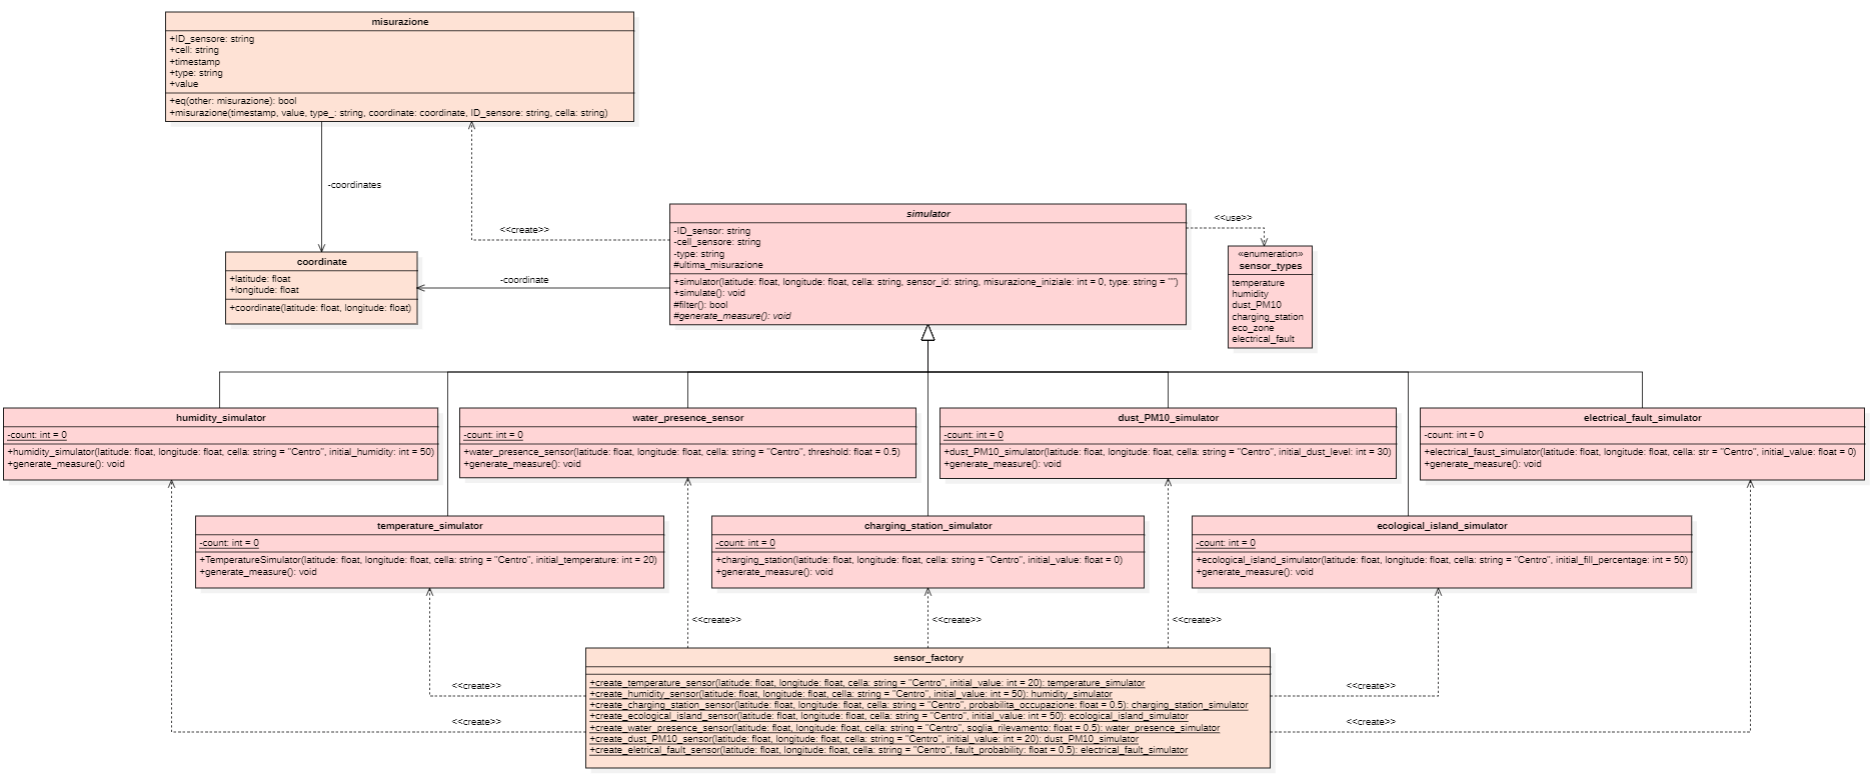
\includegraphics[width=1\textwidth]{../Images/SpecificaTecnica/simulatoriSensori.PNG}
    \caption{Modulo writers - innovacity}
    \label{fig: fdsd}
\end{figure}

Questo modulo si occupa della scrittura e/o invio di informazioni a diverse tipologie di servizi e vuole essere completamentemente indipendendente e non influenzato dal modulo della simulazione dei sensori cosi da poter consentire un suo riutilizzo.

\paragraph{Design pattern Strategy + Composite:}
Il modulo presenta un interfaccia \textit{Writer} che offre il metodo di scrittura \textit{write()} di oggetti di tipo \textit{Writable}.
Questo metodo è implementato da diverse classi concrete che rappresentano i vari servizi a cui è possibile inviare le informazioni.
Questo approccio implementa il design pattern \textit{Strategy} per la scrittura dei dati su diverse piattaforme/servizi e il design pattern \textit{Composite} per la gestione di più servizi a cui scrivere contemporaneamente in modo completamentemente indifferenziato dalla scrittura ad un singolo servizio.


L'utilizzo del design pattern Composite e Strategy in questo caso ha diverse motivazioni:
\begin{itemize}
    \item \textbf{Gestione uniforme dei servizi}: Il pattern Strategy consente di definire una famiglia di algoritmi, incapsularli e renderli intercambiabili. In questo caso, i servizi di scrittura sono trattati come algoritmi intercambiabili, consentendo di scrivere informazioni su diversi servizi senza dover conoscere i dettagli di implementazione di ciascuno.
    \item \textbf{Gestione gerarchica dei servizi}: Il pattern Composite consente di trattare gli oggetti singoli e le loro composizioni (gruppi di oggetti) allo stesso modo. Nel contesto del modulo, potrebbe esserci la necessità di gestire non solo singoli servizi, ma anche gruppi di servizi. Ad esempio, potrebbe essere utile inviare informazioni contemporaneamente a diversi servizi, come un database, un file di log e un servizio di notifica. Il Composite consente di comporre questi servizi in modo gerarchico e trattarli uniformemente.
\end{itemize}


\paragraph{Classi: metodi e attributi}


\subsubsection{Modulo Threading/Scheduling}


\paragraph{Classi: metodi e attributi}



